\subsection{Activities}

%%%%%%%%%%%%%%%%%%%%%%%%%%%%%%%%%%%%%%%%%%%%%%%%%%%%%%%%%%%%%%%%%%%%%%

\subsubsection{Hardware image acquisition}
\begin{itemize}
	\item DMA and DCMI registers were modified directly (without using any library).
	\item Hardware image acquisition allows to get full framerate (30 fps) at full resolution (VGA) into memory.
	\item Final working setup is as follows:
	\begin{itemize}
		\item External crystal oscillator (8MHz) divided by two feeds the camera, which uses its PLL to get 24MHz. This resulted in better (less noise, more squared) signals.
		\item Pin configuration from table~\ref{tab_boardpin_final} was mantained.
		\item Code can be seen at the appendix.
	\end{itemize}
\end{itemize}

\subsubsection{OV7670 register configuration}
\begin{itemize}
	\item There are some values that need to be adjusted to get a good image. For example, with the default registers the image is very sensible to light: if you point it towards something white it blanks out any other non-white color.
	\item There are many register sets floating around the internet.
	\item Different register sets yield different results and may be written to easily change between register sets (recompilation is needed at the moment).
\end{itemize}

\subsubsection{STM32-Raspberry Pi communication protocol}

\begin{figure}[ht!]
\begin{center}
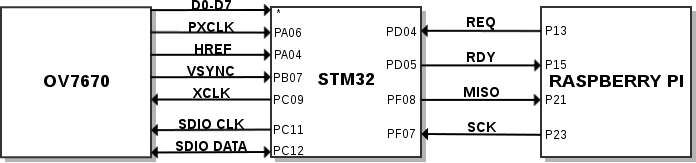
\includegraphics[height=0.22\textwidth]{fig/hwconnections}\\
\caption{Signals connected between the OV7670, the STM32 and the Raspberry Pi.}
\label{fig_hwconnections}
\end{center}
\end{figure}

\begin{itemize}
	\item Final hardware connections are shown in figure \ref{fig_hwconnections}.
	\begin{itemize}
		\item D0-D7 data lines were omitted but can be seen at table \ref{tab_boardpin_final}.
		\item Arrows indicate the data flow direction. The only bidirectional line is SDIO DATA.
		\item Transfers between the camera and the STM32 are handled by STM32's DCMI peripheral.
		\item Transfers between the STM32 and the Raspberry Pi are handled by their corresponding SPI peripherals.
		\item These are the minimal connections needed to get the image (from the OV7670) to the Raspberry Pi at a high datarate.
	\end{itemize}
\end{itemize}

\begin{figure}[ht!]
\begin{center}
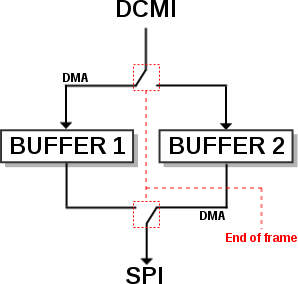
\includegraphics[height=0.45\textwidth]{fig/doublebuffer}\\
\caption{Double buffered DMA architecture. The end of frame toggles both pointers so the Raspberry always receives a full frame.}
\label{fig_doublebuffer}
\end{center}
\end{figure}

\begin{itemize}
	\item Double buffering was implemented.
	\begin{itemize}
		\item The SPI always points to the buffer the DCMI is not writing to.
		\item When a frame is completely captured, the buffers are toggled.
		\item This ensures only full and correct frames are sent to the Raspberry.
	\end{itemize}
\end{itemize}

\begin{figure}[ht!]
\begin{center}
\scalebox{1.5}{
\begin{tikztimingtable}
	REQ			& H L L 13{H} ;[dotted] 2{H}; 5{H} \\
	RDY			& H H 14{L} ;[dotted] 2{L}; 3{L} H H \\
	CLK			& L L L 13{C} ;[dotted] 2{C}; 3{C} L\\
	MISO			& U U U 18D{Image pixel data} U U\\
\end{tikztimingtable}
}
\caption{Time diagram showing the communication protocol between the Raspberry and the STM32.}
\label{fig_req_frame_time}
\end{center}
\end{figure}

\begin{itemize}
	\item A small request-response signaling needs to be performed before each transfer because the Raspberry Pi can not be the SPI slave (hardware limitation).
	\item This signaling's time diagram is shown in figure \ref{fig_req_frame_time}.
	\begin{itemize}
		\item Raspberry clears the REQ line, informing the STM32 it wants to start a SPI transfer.
		\item STM32 sets up the SPI buffer to the latest full frame and clears the RDY line.
		\item The Raspberry sets the REQ line and starts the SPI transfer.
		\item STM32 sets the RDY line when the transfer is complete.
	\end{itemize}
\end{itemize}

\subsubsection{Computer vision integration}
\begin{itemize}
	\item This task was started but there are still some things to adapt to fully run computer vision code on the received images.
\end{itemize}


%%%%%%%%%%%%%%%%%%%%%%%%%%%%%%%%%%%%%%%%%%%%%%%%%%%%%%%%%%%%%%%%%%%%%%

